\section{Architectural Design}

\subsection{Overview}
The SMURF compiler transforms a SMURF program into a playable MIDI file.
 The compiler first scans the source file, parses 
the resulting tokens, creates an abstract syntax tree, semantically 
checks the abstract syntax tree, translates the tree into 
intermediate code and finally translates this intermediate 
representation into a MIDI file which can be played in most 
media players. 


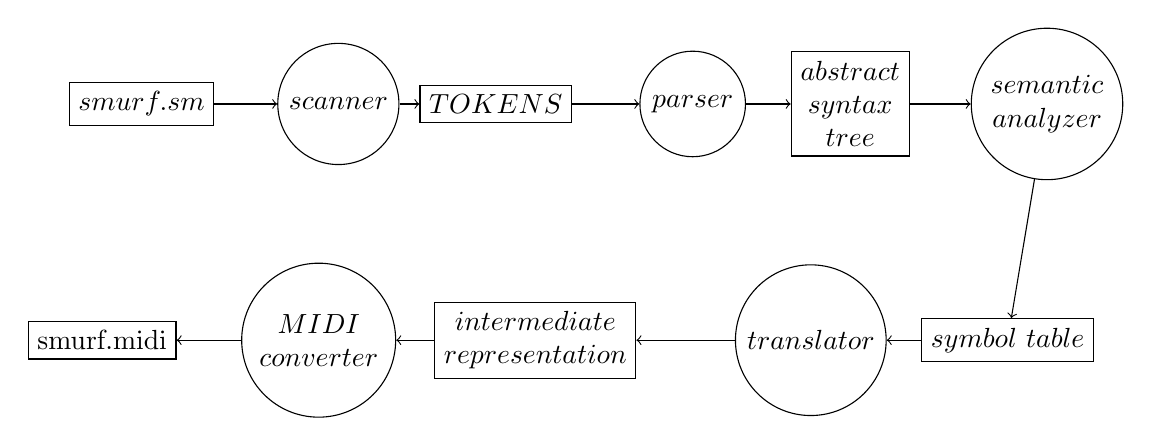
\begin{tikzpicture}[every text node part/.style={align=center}]
\node [draw,shape=rectangle] (smurf) at (0,0) {$smurf.sm$};
\node [draw,shape=circle] (scanner) at (2.5,0) {$scanner$};
\node [draw,shape=rectangle] (tokens) at (4.5,0) {$TOKENS$};
\node [draw,shape=circle] (parser) at (7,0) {$parser$};
\node [draw,shape=rectangle] (ast) at (9,0) {$abstract$ \\ $syntax$ \\ $tree$};
\node [draw,shape=circle] (semanal) at (11.5,0) {$semantic$ \\ $analyzer$};
\node [draw,shape=rectangle] (symtab) at (11,-3) {$symbol$ $table$};
\node [draw,shape=circle] (trans) at (8.5,-3) {$translator$};
\node [draw,shape=rectangle] (ir) at (5,-3) {$intermediate$ \\ $representation$};
\node [draw,shape=circle] (midic) at (2.25,-3) {$MIDI$ \\ $converter$};
\node [draw,shape=rectangle] (midi) at (-.5,-3) {smurf.midi};
\draw [->] (smurf) -- (scanner);
\draw [->] (scanner) -- (tokens);
\draw [->] (tokens) -- (parser);
\draw [->] (parser) -- (ast);
\draw [->] (ast) -- (semanal);
\draw [->] (semanal) -- (symtab);
\draw [->] (symtab) -- (trans);
\draw [->] (trans) -- (ir);
\draw [->] (ir) -- (midic);
\draw [->] (midic) -- (midi);
\end{tikzpicture}

\subsection{Scanner}
The SMURF program file is first passed to the scanner. The scanner 
matches the string of input characters to tokens and white spaces.
The tokens include keywords, constants, and operators used in a SMURF 
program. All white space characters except new lines are ignored. 
Any illegal characters are caught 
and an exception is raised. The tokens are defined with regular 
expressions and nested comments use a state machine and counter 
to be resolved. The scanner was built with the ocaml lexer. 

\subsection{Parser}
The tokens generated in the scanner are then used in the parser. 
The parser matches the string of tokens to a grammar defining the 
SMURF language. An abstract syntax tree is built as the tokens 
are matched to the grammar and stored as a program which is 
defined as a list of declarations. Syntax errors in the 
SMURF code will be identified during parsing resulting 
in an exception being raised. The parser is generated using 
the grammar and the ocaml yacc program. 

\subsection{Abstract Syntax Tree}
The abstract syntax tree is the intermediate representation 
of a SMURF program after it has been parsed but before it has 
been semantically checked. The program can easily be transversed 
by organizing the code into an abstract syntax tree because of its 
hierarchical nature. 

\subsection{Semantic Analyzer}
The semantic analyzer uses the abstract syntax tree to build a 
semantic abstract syntax tree which holds more information like 
scope and type information. Semantic errors are caught during the 
translation and transversing of the semantic abstract syntax tree. 
The semantic analyzer walked through the semantic abstract syntax tree
twice, first to create the symbol table and then to do checks using 
the filled symbol table. The second pass of the semantic abstract 
syntax tree was required because SMURF does not require variables or 
functions to be defined before they are used.  

\subsection{Translator}
The symbol table is then passed to our translator 
which evaluates all expressions and creates an intermediate 
representation that is then converted into MIDI code. 
Since symbol table contains the expression of all 
variables and functions all expressions can be evaluated 
starting from the main declaration without the semantic 
abstract symbol tree. Errors found during evaluation 
of expressions are found causing compilations errors. 
If there are no errors found then an intermediate 
representation is produced. 

\subsection{MIDI Converter}
The intermediate representation produced from the translator then 
is translated into MIDI code using the MIDI converter. The MIDI 
code can then be played. 
